\begin{figure}[ht]
  \centering
  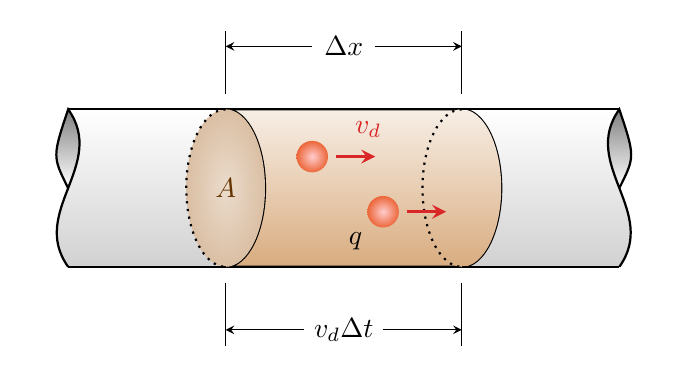
\begin{tikzpicture}[>=stealth]
    \def\rx{0.5}
    \def\ry{1}
    \def\lle{1.5}
    \def\curv{0.5}
    
    % Sombra conductor
    \shade[top color=orange!70!black!10, bottom color=orange!70!black!50] 
      (-\lle, \ry) -- (\lle, \ry)
      arc (90:-90:\rx cm and \ry cm)
      -- (-\lle, -\ry)
      arc (-90:90:\rx cm and \ry cm);

    % Sombra D (de corte)
    \shade (-\lle-2,0) .. controls (-\lle-2+\curv, 0.3) .. (-\lle-2, \ry) .. controls (-\lle-2-\curv+0.3, 0.4) .. (-\lle-2, 0);
    \shade (\lle+2,0) .. controls (\lle+2-\curv, 0.3) .. (\lle+2, \ry) .. controls (\lle+2+\curv-0.3, 0.4) .. (\lle+2, 0);

    % Sombra corte
    \shade[top color=white, bottom color=white!70!black!60] 
      (-\lle,-\ry) -- (-\lle-2,-\ry) .. controls (-\lle-2-\curv, -0.3) and (-\lle-2+\curv, 0.3) .. (-\lle-2, \ry) -- (-\lle,\ry);
    \shade[top color=white, bottom color=white!70!black!60] 
      (\lle,-\ry) -- (\lle+2,-\ry) .. controls (\lle+2+\curv, -0.3) and (\lle+2-\curv, 0.3) .. (\lle+2, \ry) -- (\lle,\ry);

    \draw[thick] 
      (-\lle, \ry) -- (\lle, \ry)
      arc (90:-90:\rx cm and \ry cm)
      -- (-\lle, -\ry)
      arc (-90:90:\rx cm and \ry cm);


    \shade[bottom color=orange!70!black!50, top color=orange!70!black!10] (\lle,0) ellipse (\rx cm and \ry cm);
    \shade[outer color=orange!60!black!36, inner color=orange!60!black!20] (-\lle,0) ellipse (\rx cm and \ry cm);

    % Sección de corte
    \draw[black,thick] (-\lle-2,-\ry) .. controls (-\lle-2-\curv, -0.3) and (-\lle-2+\curv, 0.3) .. (-\lle-2, \ry) .. controls (-\lle-2-\curv+0.3, 0.4) .. (-\lle-2, 0);
    \draw[black,thick] (\lle+2,-\ry) .. controls (\lle+2+\curv, -0.3) and (\lle+2-\curv, 0.3) .. (+\lle+2, \ry) .. controls (\lle+2+\curv-0.3, 0.4) .. (\lle+2, 0);
    \draw[black,thick] (-\lle,\ry) -- (-\lle-2,\ry);
    \draw[black,thick] (-\lle,-\ry) -- (-\lle-2,-\ry);
    \draw[black,thick] (\lle,\ry) -- (\lle+2,\ry);
    \draw[black,thick] (\lle,-\ry) -- (\lle+2,-\ry);

    \draw[thick, dotted] (-\lle,\ry) arc (90:270:\rx cm and \ry cm);
    \draw[thick, dotted] (\lle,\ry) arc (90:270:\rx cm and \ry cm);

    \node at (-\lle, 0) {\color{orange!40!black}\(A\)};

    % Cotas de medida
    \draw[thin] (-\lle,\ry+0.2) -- (-\lle,\ry+1);
    \draw[thin] (\lle,\ry+0.2) -- (\lle,\ry+1);
    \draw[thin,->] (-0.4,\ry+0.8) -- (-\lle,\ry+0.8);
    \draw[thin,->] (0.4,\ry+0.8) -- (\lle,\ry+0.8);
    \node at (0,\ry+0.8) {\(\Delta x\)};

    \draw[thin] (-\lle,-\ry-0.2) -- (-\lle,-\ry-1);
    \draw[thin] (\lle,-\ry-0.2) -- (\lle,-\ry-1);
    \draw[thin,->] (-0.5,-\ry-0.8) -- (-\lle,-\ry-0.8);
    \draw[thin,->] (0.5,-\ry-0.8) -- (\lle,-\ry-0.8);
    \node at (0,-\ry-0.8) {\(v_d \Delta t\)};

    % Cargas
    \shade[inner color=white!80!red, outer color=orange!50!red!70!lightgray] (-0.4,0.4) circle (.2) [radius=1pt];
    \draw[very thick,color=red!70!gray,->] (-0.1,0.4) node[above right=3pt] {\(v_d\)}-- (0.4,0.4) ;
    \shade[inner color=white!80!red, outer color=orange!50!red!70!lightgray] (0.5,-0.3) node[below left=4pt] {\(q\)} circle (.2) [radius=1pt];
    \draw[very thick,color=red!70!gray,->] (0.8,-0.3) -- (1.3,-0.3);
  \end{tikzpicture}
  \caption{Movimiento de cargas en un conductor.}
  \label{fig_movimiento_de_cargas}
\end{figure}
